\documentclass[tikz]{standalone}
\usepackage[T1]{fontenc}
\usepackage{newtxtext}
\usepackage[smallerops]{newtxmath}
\begin{document}
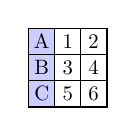
\begin{tikzpicture}
\tikzstyle{every node}=[draw, scale=0.75, inner sep=0mm]
\tikzstyle{matrix of nodes}=[
inner sep = 0mm,
execute at begin cell=\node\bgroup,
execute at end cell=\egroup;%
]
\tikzstyle{column 1} = [nodes={fill=blue!20}]
\matrix [matrix of nodes, nodes={draw, inner sep=0pt, anchor=center}, minimum size = 1.25em,
row sep=-\pgflinewidth, column sep=-\pgflinewidth,
column 1/.style={nodes={fill=blue!20}}]
{
A & 1 & 2 \\
B & 3 & 4 \\
C & 5 & 6 \\
};

\end{tikzpicture}
\end{document}
